At the end of this worksheet you should be able to  
\begin{itemize}
	\item describe the quantities involved in discussing rotational motion and the connection of them to translational motion.
	\item calculate the quantities describing rotational motion.
	\item use the conditions of equilibrium to solve for an unknown quantity.
	\item use the principle of conservation of angular momentum to solve for an unknown quantity.
\end{itemize}


\begin{enumerate}
	\setlength\itemsep{1 in}
	
	\item
	In the lecture video, I talked about the analogy between linear (translational) motion and rotational motion. All of the most important equations that we have used have a corresponding version in rotational motion. I wrote down in the notes many of these rotational version, but I skipped over the kinematic equations so let's do them here. I am not interested in you working with these equations since we have conservation of energy and conservation of angular momentum now, but do this as an exercise in understanding the analogy. 
	
	\item
	You exert a force of 100N to open a door. To get the door swinging you exert this force for 1 second and you apply this force perpendicularly to the door. The door is 1m wide and 2m tall and has a mass of 30kg. The door handle is 0.9m from the hinges. 
	\begin{itemize}
		\setlength\itemsep{1 in}
		\item What torque do you exert on the door?
		\item What is the rotational inertia of the door? $I=\frac{1}{3}ML^2$
		\item What is the angular acceleration of the door?
		\item How fast is the door moving when you stop pulling and let it swing?
		\item What is the initial angular momentum of the door? What angular impulse did you give the door? 
		\item What is the door's final angular momentum? Use this to find the angular speed when you stop changing the door's momentum.
		\item What is the door's kinetic energy after you stop pulling?
		\item What was its initial kinetic energy? How much work did you do to open the door?
		\item Over what angular displacement did you exert this 100N force?
		\item I can't think of anything else to calculate about this; can you?
	\end{itemize}
	
	\item 
	Look up and estimate the rotational inertia of some objects around you. I see a basketball, a book, an iPad, a car tire, and a barbell. Pick some objects and look up their dimensions and calculate their rotational inertia.
	
	\item
	Let's calculate the rotational inertia of the demonstration apparatus that I used in the video.
	This is a compound shape, but we only need to add together the individual rotational inertia of each. Also since the point masses on the rods and the rods themselves are repeated 4 times around the device, we just need to find that once and multiply by 4. The pulley in the center is 4 discs stacked together, so we will model each one and add them together.\\
	
	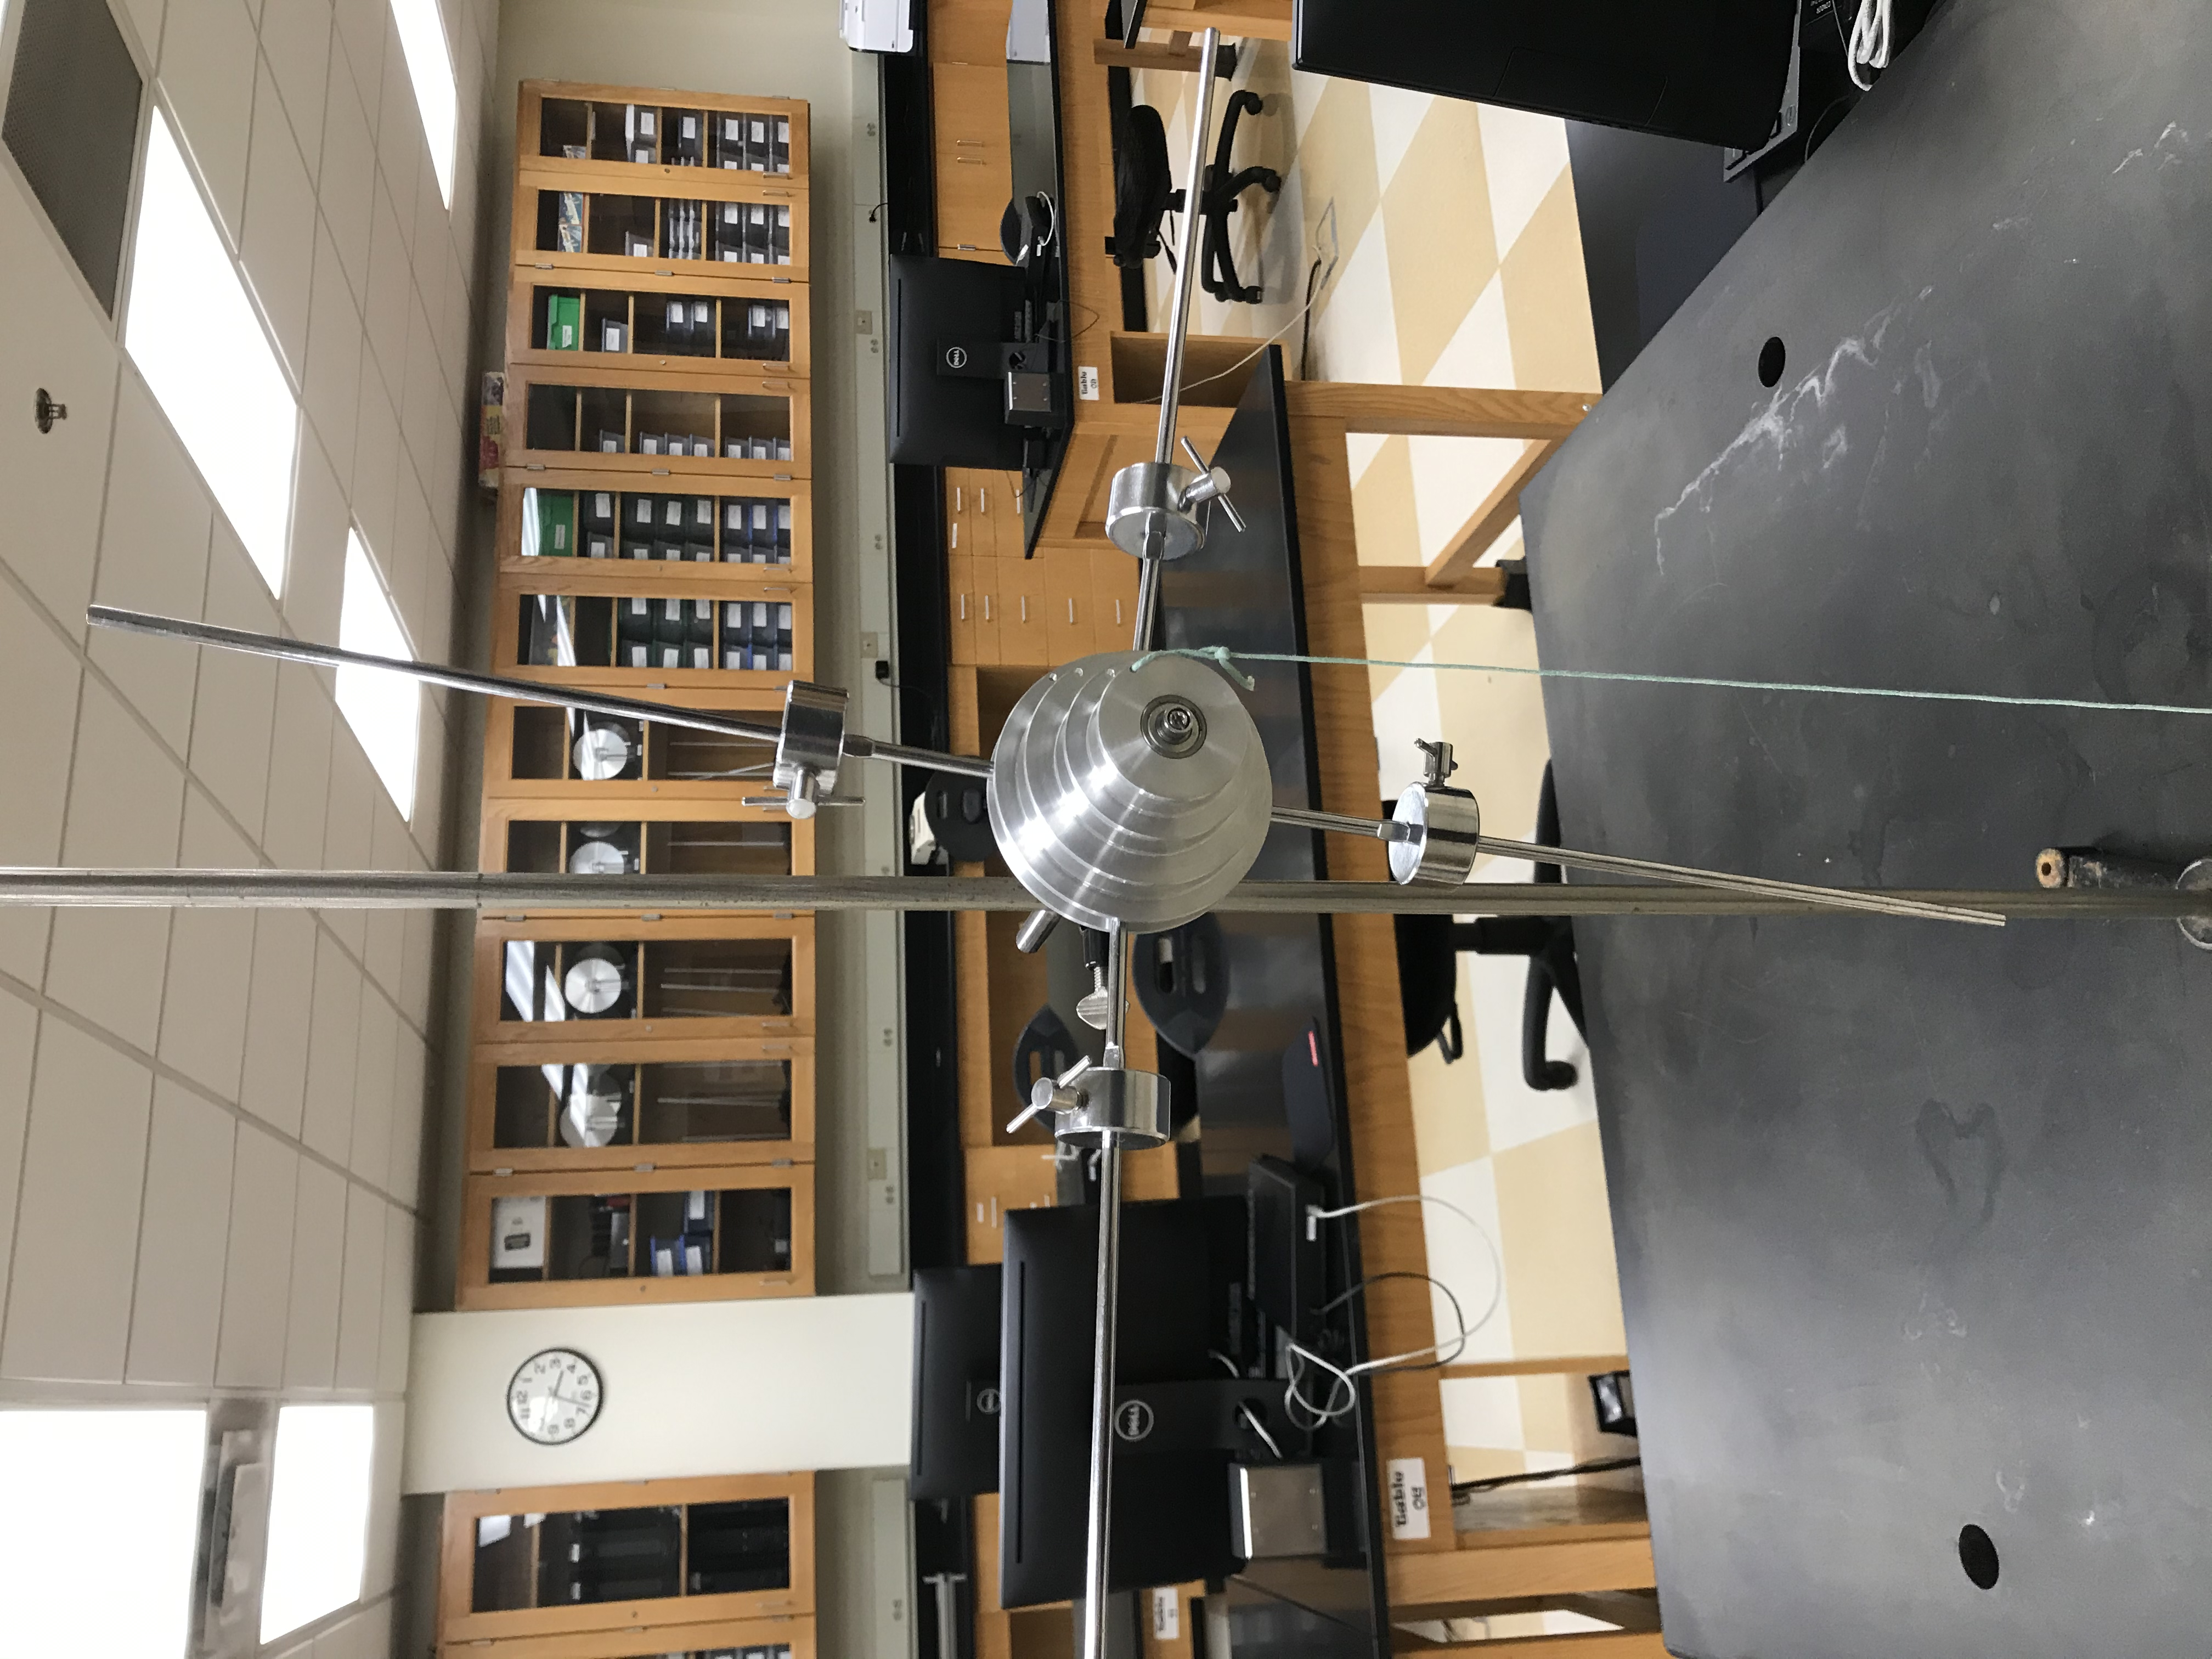
\includegraphics[scale=.09, angle=-90]{2020-10-16_15.33.07.jpg}
	
	\item
	In lab this week, we will measure the rotational inertia of a disk and also of a hollow cylinder. To do this we will apply a constant torque to a pulley below the spinning object and measure the angular acceleration of the spinning object. To apply a constant force to the pulley, we will use a mass that will hang down from a string and have a constant force of gravity applied to it. Lets do this problem \emph{in general} and develop an equation to calculate the rotational inertia from knowing the hanging mass, the radius at which the string is applying a torque to the pulley. \emph{Be careful here! The force applied to the pulley is not $mg$. The hanging mass is accelerating, but not with \SI{9.8}{m/s^2}}\\
	Some starters:
	\begin{itemize}
		\item Draw a free body diagram on the hanging mass. You know the weight but you do not know the tension. 
		\item In lab we will measure the angular acceleration, so how can we write the acceleration fo the hanging mass in terms of the angular acceleration of the spinning pulley its attached to?
		\item 
	\end{itemize}
	\giantskip
	
	\item
	To generate torque with a wrench, you exert a force at the end of the wrench, 30cm away from the bolt. You push with 500N in the direction to loosen the bolt, but it will not budge. Why is it not rotating? In order to generate more torque, you go get a longer wrench, this one 55cm. You can still only push with 500N of force, so how much torque have you applied now? By what factor have you changed the length of the lever arm? By what factor have you changed the torque?\hugeskip
	
	\item
	A person laying on the floor is doing a leg lift with an ankle weight on. The ankle weight is 50 N. Explain why the exercise is hard at first when the leg is horizontal but very easy when the leg gets to vertical. Find the torque on the persons leg when their leg is at \ang{30} with respect to the horizontal. The ankle weight is essentially at the end of their leg which is 1m long, and the mass of their leg is 12.75kg. Take the center of mass of the leg to be the geometric center of the leg. Calculate this again when their leg is at an \ang{80} with respect to the horizontal.\hugeskip
	
	\item
	Two people are carrying a 1000N wooden beam that is 5m long. One person is positioned at one end of the beam, and the other person is positioned 1m away from the other end. What force is each person exerting on the beam?\hugeskip
	
	\item 
	Let's do the previous problem inside out. A question might read, ``Where should the second person be positioned so that his force on the beam is \blank?'' Provide the force from the previous question and solve for his position from one end.
	
	\item 
	Another followup, where would the second person need to be so that his force was 750 N?\hugeskip
	
	\item
	Chris and Jamie are carrying Wayne on a horizontal stretcher. The uniform stretcher is 2.00 m long and weighs 100 N. Wayne weighs 800 N. Wayne's center of gravity is 75.0 cm from Chris. Chris and Jamie are at the ends of the stretcher. What force is Chris providing to support the stretcher? What force is Jamie providing to support the stretcher?\hugeskip
	
	\item
	A pole-vaulter holds out a 4.75m pole horizontally in front of him. Assuming the pole is uniform in construction, and that he holds the pole with one hand at the very end, and one hand 0.75m from the end, what is the ratio of the force applied by the hand on the end of the pole to the weight of the pole?\hugeskip
	
	\item
	Will wants to hit a PR in bench press. His target total weight is 147.5lbs. The bar is 45lbs, and he has two 45 lb plates, two 10lb plates, two 5lb plates, and two 2.5 lb plates to choose from. This collection of plates cannot be made into 147.5lbs shared symmetrically on both sides. Determined to hit his PR, he puts 50lbs on one side of the bar, and 52.5 lbs on the other side. He thinks that he can grip the bar off center, and apply the same force to the bar as he would have if he had a combination of plates that would allow the weight to be evenly distributed. His spotter John is skeptical that this will work and it sounds dangerous, so they come to you to solve the problem. The weights are 5 ft apart and can be treated like point masses. He likes to grip the bar with his hands two feet apart. Can he lift this weight with the same force on both hands and if so how far should he position his hands off center? \emph{Don't worry about any conversions to metric here. Pounds are already a force and multiplying them by feet gives foot-pounds, which is the US customary system units of torque.}

	
\end{enumerate}